\chapter{Detecting Contamination in massive parallel sequencing studies}
\label{chapterContamination}
With the new technological progress that comes with the DNA sequencing based on massive parallel sequencing, there are however also some drawbacks. The shorter read-length compared to Sanger-based Sequencing can be targeted with the so called Third Generation Sequencing, with new companies like Oxford Nanopore Technologies\footnote{\url{nanoporetech.com}}, Pacific Biosciences\footnote{\url{http://www.pacb.com/}} or BioNano Genomics\footnote{\url{http://bionanogenomics.com/}} already conquering the market for sequencing devices. Another issue, that becomes more prevalent, is the immanent issue of contamination, based on the very sensitive NGS technology. While Sanger based Sequencing is able to detect heteroplasmic variants down to the 10\% level for the minor allele \cite{Kloss-Brandstatter2015}, NGS can detect heteroplasmic variants down to the 1\% minor allele level and even lower \cite{Li2010}. Also the expanding amount of sequencing studies increases the probability of errors to occur. The error can come in many forms in the lab, but also in the data processing steps. While in the lab or while sequencing, sample contamination, cross-species contamination, carry-over contamination from previous run, issues with PCR products, issues with fragmentation of DNA, wrong protocols and many more can become problematic. The post-processing from the raw sequencing reads to the annotated variants can also lead to errors, due to wrong methods applied, with the wrong parameters, wrong reference sequences in use (this is especially the case for mitchondrial sequencing studies where different reference sequences are in use \cite{Behar2012,Andrews1999} or systematic errors as previously described (see phantom mutations \ref{}). One option to avoid post-processing errors, is the use of automated pipelines, reducing the risk such issues. Quality control is a second important option. Therefore in this chapter the concepts described in Chapter \ref{chapterHaploGrep} and Chapter \ref{chaptermtDNA-Server} get combined to check mitochondrial data derived from massive parallel sequencing for the presence of contamination, based on low-level heteroplasmy that can be used to help identifying an extra haplogroup in the sample of interest (see section \ref{haplochecker}. The concept was drafted in Li et al \cite{Li2010} based on manual inspection with Phylotree as well as in Avital et al \cite{Avital2012} by taking advantage of HaploGrep. A recent discussion highlights the problem of contamination in mitochondrial NGS studies \cite{Ye2014,Just2014, Just2015,Ye2014reply} and tools for detection of contamination are emerging \cite{Renaud2015,Jun2012,Dickins2014}, as presented in the related work section \ref{cont:relatedwork}. The performance of the new workflow called HaploChecker is presented in the Results section \ref{cont:result}, and the method is abstracted in the last section \ref{cont:outlook}, by highlighting future applications as well as opportunities for improvements.

\section{Related Work}\label{cont:relatedwork}
The need for a quality check of sequencing data has been addressed in the past for Sanger based data \cite{Walker2004, Montesino2007, Bandelt2009, Yao2007} as well as for NGS based data \cite{Holland2011}. 
Concepts for detecting and correcting contamination were presented for nuclear DNA NGS sequencing projects, where MicroArray data are available were presented in Jun et al. \cite{Jun2012} and Flickinger et al. \cite{Flickinger2015} respectively. The provided application \textbf{VerifyBamId}\footnote{\url{http://genome.sph.umich.edu/wiki/VerifyBamID}} is applying likelihood-based methods for detecting sample contamination based on sequence and MicroArray-based genotype data \cite{Jun2012}. This approach was applied on all samples from the 1000 Genome data set, and the resulting data release Phase 1 and Phase 3 were filtered accordingly the contamination-index provided by VerifyBamID. 

A recent approach was presented by Dickins at al. \cite{Dickins2014} by describing a Galaxy \cite{Goecks2010,Afgan2016} based pipeline for contamination control in mitochondrial genomes. The pipeline as well as the data are available through the website\footnote{\url{https://usegalaxy.org/u/aun1/p/controlling-for-contamination-in-resequencing}}. An advantage of this tool is the Galaxy related reproducibility of the workflow. See Appendix for the graphical representation of the workflow \ref{app:galaxy-workflow}. The concept of the method is based on building a Neighbor-Joining (NJ) tree \cite{Saitou1987}, for the minor allele frequency (MAF). The method is based on the assumption that contamination is manifested in a sample by multiple polymorphic sites with tight MAF distribution. The provided workflow is straightforward in small to large scale data sets such as in population studies. While this approach can have advantage over a haplogroup-based detection of contamination in some situations, it is not suitable for investigations on single profiles which accounts in particular for forensic investigations but also for case studies in medical research. Further the source of contamination is required to be present in the data set, often not feasible.

A further different approach is presented in the tool called \textbf{Schmutzi} by Renaud et al. \cite{Renaud2015}, for detecting contamination in ancient mitochondrial DNA samples. Based on empirical and simulated data sets, the contamination estimation tool is designed for highly degraded mtDNA also affected by cytosine deamination (loosing an amine group from the molecule, being  a process typical in ancient DNA) and problems with contamination with present day DNA.  However, the absence of deamination yields incorrect estimations and therefore their tool is highly recommended to be used exclusively on mtDNA harbouring the mentioned properties. The underlying framework is based on a Bayesian maximum a posteriori algorithm, which yields the most likely model parameters from the provided data. 

While the presented related tools are designed for different NGS derived data, the comparison with our new method is performed on two different data sets. For comparison with the mitochondrial NGS data, we compare the data set provided by Dickins et al. \cite{Dickins2014} to check if the haplogroup-based contamination check presented subsequently can detect the expected contamination described. We further demonstrate the use of our approach in the 1000 Genomes phase 3 data set, including 2,504 whole genome sequences from 26 populations world wide. A direct comparison with the tool from Renaud et al. could not be performed.


\section{mtDNA phylogenetic approach for contamination control}\label{haplochecker}
We developed a tool for mitochondrial sequence data analysis for estimation of contamination accessible via http://mtdna-server.uibk.ac.at/start.html and as a standalone version on Github https://github.com/haansi/greenVC. The underlying principle is that all mitochondrial variants relative to the mitochondrial reference sequence rCRS \cite{Andrews1999} can be split into minor and major variant allele frequency (VAF), as suggested by Li et al. \cite{Li2010} and Avital et al. \cite{Avital2012}.
\subsection{Naive Variant Caller}
While the method presented in Chapter \ref{chaptermtDNA-Server} directly implements the approach presented in \ref{cont:haplochecker}, it was not designed for the purpose of detecting low-level contaminations in low-coverage data, but rather detect reliably the presence of homo- and heteroplasmic variants. To detect contamination below the 10\% level in sequence data with a coverage $<$ 100 fold, a naive variant caller was designed, based on the HTSJDK framework\footnote{\url{https://samtools.github.io/htsjdk/}}, and applies a Clopper Pearson binomial confidence interval \cite{CLOPPER1934}, representing an exact confidence interval. The number of minor alleles (x), the coverage (n) and the confidence level ($\alpha$) are provided, such that the lower limit ($ll$) and upper limit ($ul$) are provided:
\begin{equation}
 ll = \frac{1}{(1 + \frac{(n - x + 1)}{(x qf(\frac{\alpha}{2}, 2 x, 2 (n-x+1)))})}
\end{equation}
\begin{equation}
 ul = \frac{1}{(1 + \frac{(n - x)    }{ ((x + 1)  qf(1-\frac{\alpha}{2}, 2 (x+1), 2 (n-x)))})}
\end{equation}
For $x=0$ yields $ll=0$ and $ul = 1 - (\frac{\alpha}{2})^{(\frac{1}{n})}$ and for $x = n$ $ll = \frac{\alpha}{2}^{(\frac{1}{n})}$, and $ul =1$. Since those two exceptions represent homoplasmic variants (either all bases according the reference or all bases as complete exchange), the calculation can be omitted.
The quantile function $qf$ accepting the quantile parameters for the F-distribution ( $ll_{\alpha} = \frac{\alpha}{2}$ and $ul_{\alpha}= 1-\frac{\alpha}{2}$ respectively) and the degrees of freedom ($ll_{df_1} = 2x$, $ll_{df_2} = 2 (n-x+1)$,  $ul_{df_1} =  2 (x+1)$, $ul_{df_1} =  2 (n-x)$ ) \footnote{\url{https://stat.ethz.ch/R-manual/R-devel/library/stats/html/Fdist.html}}. A heteroplasmy is marked as reliable, when the lower limit exceeds the user defined threshold $h_T$ ($ll  \geq h_T$). The Clopper-Pearson implementation from the Apache Commons Mathematics Java Library\footnote{\url{http://commons.apache.org/proper/commons-math}} is applied.
\begin{enumerate}
\item \textbf{bam2var}: a user defined quality score filtering is applied, and all reads with read length $>$ 20 bases are considered. Reads are handled in such manner, that the circular structure of the mtDNA is considered, and positions exceeding the length of the user-provided reference restart at base 1. 
The parameters are the BAM input file (in), the result folder (out), where the pileup file as well as the variant file and haplogrep input files are generated, the reference sequence (ref), the variant allele frequency (VAF), applied to distinguish between heterop, and homoplasmic variants and the base quality (QUAL). The listing shows an example, VAF corresponding to 20\% here:
\begin{lstlisting}[language=bash]
java -jar greenVC.jar bam2var --in HG01500.IBS.exome.MT.bam --out resultfolder  --ref data/rcrs.fasta  --VAF 0.2 --QUAL 20
\end{lstlisting}
\item \textbf{haplocheck}: generation of the haplogrep input files for contamination detection. The method is presented in \ref{cont:haplochecker}. This command writes based on the previous called variants to a haplogrep input file, by splitting it in major/ minor allele profiles in order to check for sample contamination down to the 5\% heteroplasmic level.
\begin{lstlisting}[language=bash]
java -jar greenVC.jar haplocheck --in resultfolder/variants.txt --out haplogrepinput.hsd   --VAF 0.05 
\end{lstlisting}
\item \textbf{haplocheck-mtDNA-Server}: the result in the heteroplasmies.txt file from mtDNA-Server (see Chapter \ref{chap:NGS}) is handled similar to the \textbf{haplocheck} option. Again, the input file is assigned major/ minor allele profiles in order to check for sample contamination with HaploGrep \ref{chapterHaplogrep}. Example call:
\begin{lstlisting}[language=bash]
java -jar greenVC.jar haplocheck-mtDNA-Server --in heteroplasmies.txt --out haplogrepinput.hsd  --VAF 0.05 
\end{lstlisting}
\item \textbf{lofreq}: the resulting VCF file, generated by LoFreq \cite{Wilm2012}, as an additional ultra-sensitive variant caller (able of calling variants occurring in <0.05\% of all reads) can further be used as data input. The htsjdk-library\footnote{\url{https://github.com/samtools/htsjdk}} is applied here to read the VCF file, and transforming the information provied to HaploGrep input profiles. LoFreq itself does not call genotypes\footnote{\url{http://csb5.github.io/lofreq/}}, so the SAMPLE and FORMAT columns in the VCF file are missing.The required information for the generation of HaploGrep files, are the vcf filename, the position, the reference and the alternative base, as well as the allele frequency, provided in the INFO
\begin{lstlisting}[language=bash]
java -jar greenVC-0.1.jar lofreq --in inputfile.vcf --out haplogrepinput.hsd 
\end{lstlisting}
\item \textbf{GUI}: the application has a simple Swing GUI, shown if no parameter is provided. The bam2var step is calculated based on the parameters previously described.
\end{enumerate}
The presented method requires manual inspection of the HaploGrep results, while this is not explicitly the case for the pipeline presented thereafter. 
\subsection{HaploChecker}\label{cont:haplochecker}
Haplochecker starts with the called pileup variant file, with the variants in tab-spaced fileformat. Shared homoplasmic mutations help identifying the source of contamination, indicating mutual variants along phylogenetic branches. The contamination detection approach is also implemented directly in mtDNA-Server pipeline as drafted in Chapter \ref{chap:NGS} for FASTQ or BAM files. On the web interface again generated by Cloudgene, files for upload are requested to include the following indications: Sample ID (ID), mtDNA Position (POS), Major Allele (WTALLELE), Variant Allele (MUTALLELE) and the minor variant allele frequency (VAF). The threshold for heteroplasmy level detection is user defined and is employed to differentiate between heteroplasmic and homoplasmic variants. After the file upload is performed, HaploGrep  profiles are generated directly in the pipeline by separating the minor and major component of a heteroplasmic variant accordingly to the resulting profiles (Figure ). HaploGrep is based on the constantly updated worldwide mtDNA phylogeny Phylotree of currently 5,437 haplogroups. The generated profiles are subsequently checked for haplogroup (hg) consistency. The generated report indicates possible contaminations based on phylogenetic differences. Figure \ref{cont:workflow} represents the overview of this workflow. It is possible to provide both either heteroplasmic and homoplasmic sites or heteroplasmic sites only. The differing haplogroup affiliations of major and minor component are reported per sample along with a score value indicating the following additional information: a) heteroplasmies found in the resulting haplogroup, b) positions not covered under this haplogroup affiliation, c) heteroplasmies not showing any impact on the current phylogeny (either according the rCRS or never observed in Phylotree 17) (global private mutations) or heteroplasmiesic variants found in other haplogroups (local private mutations). For all polymorphisms found in the resulting haplogroup, the standard deviation and the mean value of the VAF of heteroplasmic mutations are calculated, and the results are represented as boxplots (see Appendix). 
\begin{figure}[!ht]
    \centering
    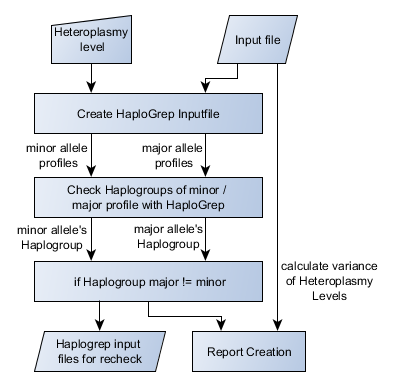
\includegraphics[width=0.8\textwidth]{images/dataflow.png}
    \caption[Pipeline for contamination detection]{Pipeline for contamination detection } 
    \label{cont:workflow}
\end{figure}

 
\section{Results}\label{cont:result}
The pipeline was defined as a YAML file for the generation of the Cloudgene based workflow, abstracted in the Figure \ref{cont:workflow}. The workflow joins two JAR files, one for the generation of the HaploGrep profiles and the second representing a console version of HaploGrep, as well as the logic for contamination detection directly implemented in R, accepting the HaploGrep result files, and the input files for the generation dynamic html report, based on R Markdown. 
The download of the chromosome MT BAM files resulted in a data volume of 97 GB. In total 2,504 samples were analyzed, as inferred from the sample information provided on the public available sample information (see Supplemental Material for URL). Supplemental Table 1 displays the mapping statistics over all 2,504 samples. In total 1,174,564,365 reads were processed on mtDNA-Server with the previously described parameters yielding to 12,489 heteroplasmic sites over all samples, corresponding 4.98 heteroplasmies per sample. The frequency of the highest occurring mtSNPs is corresponding the expected hot spots in the mitochondrial genome – See supplemental Table 2. Heteroplasmies are manifested on 5,065 sites out of all possible 16,569 sites. 

\subsection{Validation}
The evaluation of Haplochecker  was performed using simulated data, where we randomly mixed haplotypes of known haplogroups in silico and generated test profiles. As contamination detection within haplogroup H (approximately 45\% within Europe) is critical due to the comparison or largely similar sequences according to the European reference (rCRS), we placed particular emphasis on the validation of sequences belonging to haplogroup H. Therefore, we mixed all neighboring samples assigned to haplogroup H (858) and again generated test profiles (see supplemental Materials). Subsequently, the major and minor profiles of the haplotypes were retrieved by assigning different variant allele frequencies for each shared, minor and major mutations. Shared mutations were denoted with VAF 1, major variants $>$0.5 and minor contributions $\leq$ 0.5), respectively. For these simulations, we used data of the most recent phylogeny based on Phylotree 17, comprising 4,560 variants (3,740 transitions, 399 transversions, 50 inserts, 50 deletions and 123 back mutations defining 5,435 haplogroups. 
\subsection{1000G phase 3 data}
The data previously described and processed by the pipeline shows several samples with a high number of heteroplasmic variants $\geq$ 20 sites. Large amount of those samples can be identifies as contaminated (see Figure \ref{cont:1000G}). What further gets visible in this experiment, is the coverage distribution over the 2,504 samples. A cluster becomes apparent that has a low coverage of $\leq$ 500x coverage. Since all data are generated by whole genome sequencing on the same vendor's devices, the coverage reflects the relative amount of mitochondrial copy number to the nuclear DNA. Taking the provided 1000G sample information into account, the variance in the mean coverage can be explained by the origin of the DNA extraction. Samples with DNA extracted from blood show a much lower mitochondrial copy number (mtCN) compared to samples where the DNA was extracted from the lymphoblastoid cell lines (LCL). The mitochondrial copy number is often calculated as $m$ or $mtCN$, by calculating the ratio between reads mapping to the mitochondrial genomes ($r_m$), to the reads which map to the nuclear genome ($r_n$)\cite{Reznik2016}.
\begin{equation}
mtCN = \frac{r_m}{r_n}
\end{equation}
Ding et al \cite{Ding2015} further take the two copies of autosomal DNA in the cell into account, by taking the average coverage of the mtDNA ($avgCov_m$) and the autosomal DNA ($avgCov_n$) into account:
\begin{equation}
mtCN = \frac{avgCov_m}{avgCov_n}\times{2}
\end{equation}
When making statements about the copy number derived in this manner, it is of extreme importance not to mix samples where different DNA extraction methods are applied.
\begin{figure}[!ht]
    \centering
    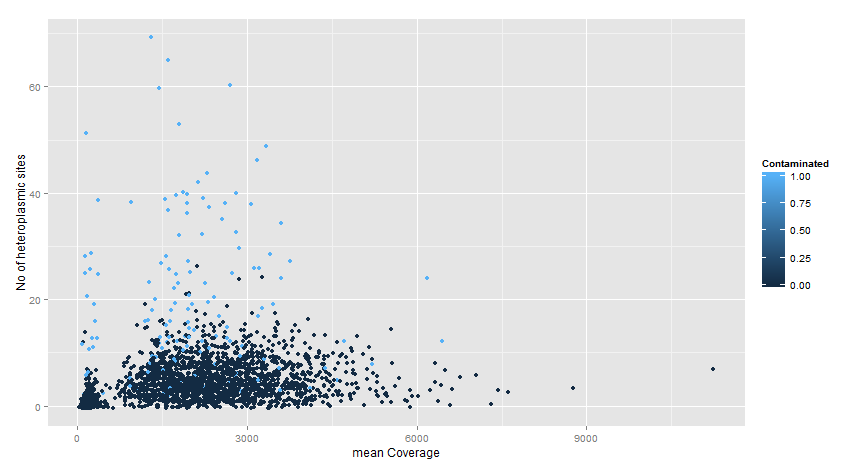
\includegraphics[width=1\textwidth]{images/contamination1000g.png}
    \caption[Contaminated Samples in 1000G phase 3]{Contaminated Samples in 1000G phase 3, the x-axis represents the mean coverage per sample, and the y-axis represents the amount of heteroplasmic sites per sample. The color indicates if a sample is affected by contamination.} 
    \label{cont:1000G}
\end{figure}
\subsection{Pipeline Performance Comparison}
While the direct comparison to the method from Renaud et al. \cite{Renaud2015} is not feasible for non-degraded DNA, the comparison to the Galaxy pipeline \cite{Dickins2014} as well as the VerifyBamId \cite{Flickinger2015} is represented in this subsection. The different setups for the comparison are the following: 
\begin{itemize}
\item The data represented in \cite{Dickins2014} was downloaded resulting in 13GB of paired end FASTQ files. The processing of the data was done with a private mtDNA-Server installation, and the samples were assessed for contamination with the herein presented method. Subsequently the results from Dickins et al were compared. Figure \ref{cont:family} summarizes the contaminated samples in the data provided by Table \ref{comptable} represents the results from the Galaxy Pipeline and the results from the contamination pipeline directly implemented in mtDNA-Server.
\begin{figure}[!ht]
    \centering
    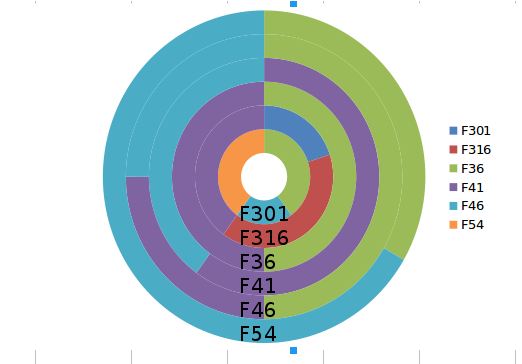
\includegraphics[width=0.7\textwidth]{images/families.png}
    \caption[Contamination represented in the Family mtDNA data]{Contamination represented in the Family mtDNA data  \cite{Dickins2014} analyzed with the herein described method regarding contamination. As can be seen, the different families F301 (n=5), F316 (n=5), F36 (n=6), F41 (n=5), F46 (n=4) and F54 (n=3) all show traces of contamination. Each circle represents a family, the color represented in the legend indicate what other DNA contributed the contaminations.} 
    \label{cont:family}
\end{figure}
\begin{table}[]
\centering
\caption{Comparison Galaxy pipeline to the contamination detection based on the known phylogeny implemented in mtDNA-Server. Total.Sites represents the heteroplasmic variants found in each sample, EVAL for the Galaxy Pipeline are classified in fail (contaminated), warn (possible contamination) and pass (no contamination). EVAL for mtDNA-Server lists a haplogroup, indicating the source of contamination if present, or empty, if the Total.Sites can not be assigned a minor profile. Samples highlighted in blue indicate the contaminated ones, samples in orange indicate conflicting results between the two pipelines.}
\label{comptable}
\begin{tabular}{lllll}
     & \multicolumn{2}{c}{\textbf{Galaxy}} & \multicolumn{2}{c}{\textbf{mtDNA-Server}} \\
\textbf{Sample}       & \textbf{Total.Sites}     & \textbf{EVAL}     & \textbf{Total.Sites}        & \textbf{EVAL}        \\
F301-M468-BL &35 &\cellcolor[HTML]{34CDF9} fail &30 &\cellcolor[HTML]{34CDF9}H3af \\
F301-M468C1-BL &40 &\cellcolor[HTML]{34CDF9} fail &45 &\cellcolor[HTML]{34CDF9}H3af \\
F301-M468C2-BL &47 &\cellcolor[HTML]{34CDF9} fail &47 &\cellcolor[HTML]{34CDF9}K2a10 \\
F301-M468C3-BL &33 &\cellcolor[HTML]{34CDF9} fail &51 &\cellcolor[HTML]{34CDF9}K2a10  \\
F301-M468C4-BL &39 &\cellcolor[HTML]{FFCC67}warn &64 &\cellcolor[HTML]{34CDF9}U2e2a1 \\
F316-M483-BL &38 &\cellcolor[HTML]{34CDF9} fail &65 &\cellcolor[HTML]{34CDF9}J1b1a1a \\
F316-M483C1-BL &41 &\cellcolor[HTML]{34CDF9} fail &46 &\cellcolor[HTML]{34CDF9}J1b1a1a \\
F316-M483C2-BL &25 &\cellcolor[HTML]{34CDF9} fail &31 &\cellcolor[HTML]{34CDF9}J1c1a \\
F316-M483C3-BL &8 &warn &3 & \\
F316-M483C4-BL &6 &warn &0 & \\
F36-M45-BL &5 &pass &1 & \\
F36-M45C1-BL &8 &warn &0 & \\
F36-M45C2-BL &7 &warn &3 & \\
F36-M45C3-BL &43 &\cellcolor[HTML]{34CDF9} fail &38 &\cellcolor[HTML]{34CDF9}J1b1a1a \\
F36-M45C4-BL &42 &\cellcolor[HTML]{34CDF9} fail &39 &\cellcolor[HTML]{34CDF9}J1b1a1a \\
F36-M46-BL &12 &\cellcolor[HTML]{34CDF9} fail &41 &\cellcolor[HTML]{34CDF9}J1b1a1a \\
F41-M51-BL &9 &warn &13 &\cellcolor[HTML]{FFCC67}J1b1a \\
F41-M51C1-BL &6 &warn &2 & \\
F41-M51C2-BL &7 &warn &2 & \\
F41-M52-BL &54 &\cellcolor[HTML]{34CDF9} fail &59 &\cellcolor[HTML]{34CDF9}U2e2a1 \\
F41-M52C1-BL &39 &\cellcolor[HTML]{34CDF9} fail &52 &\cellcolor[HTML]{34CDF9}U2e2a1 \\
F46-M57-BL &46 &\cellcolor[HTML]{34CDF9} fail &59 &\cellcolor[HTML]{34CDF9}J1b1a1a \\
F46-M58-BL &12 &warn &18 & \\
F46-M58C1-BL &43 &\cellcolor[HTML]{34CDF9} fail &36 &\cellcolor[HTML]{34CDF9}H3af \\
F46-M58C2-BL &35 &\cellcolor[HTML]{34CDF9} fail &36 &\cellcolor[HTML]{34CDF9}H3af \\
F54-M67-BL &37 &\cellcolor[HTML]{34CDF9} fail &32 &\cellcolor[HTML]{34CDF9}H3af \\
F54-M67C1-BL &44 &\cellcolor[HTML]{34CDF9} fail &58 &\cellcolor[HTML]{34CDF9}U2e2a1 \\
F54-M67C2-BL &42 &\cellcolor[HTML]{34CDF9} fail &51 &\cellcolor[HTML]{34CDF9}U2e2a1  \\       
\end{tabular}
\end{table}

\item The Phase 3 data released was verified with VerfifyBamID prior to publication by the 1000G consortium\footnote{\url{http://ftp.1000genomes.ebi.ac.uk/vol1/ftp/technical/working/20130514_phase3_verifybam_results/}}. For verifying the herein presented haplogroup based contamination detection approach, the mitochondrial sequences were downloaded from all samples marked with the verdicts \verb|HIGH_CHIP_MIX| (n=27), \verb|HIGH_FREE_MIX| (n=11) and \verb|POSSIBLE_SWAP| (n=7) from the FPT site \footnote{\url{ftp://ftp.1000genomes.ebi.ac.uk/vol1/ftp/data_collections/1000_genomes_project/data/}}. The data comprised 37 CRAM\footnote{http://www.ebi.ac.uk/ena/software/cram-toolkit} files (8 samples showed two verdicts), and was retrieved with the latest Samtools 1.3.1. In a second step the CRAM files were converted to FASTQ files and remapped with BWA MEM to the rCRS reference sequence. Thereafter all steps were identical to the analysis of the 1000G Phase 3 low coverage data described previously.
The file size of the samples accumulated to \~ 500 MB, varying significantly in size. The mean coverage over the mt-genome varies between \~100x (HG03982) and \~8,000x (HG03799). Out of the 3 different contamination classifications (\verb|HIGH_CHIP_MIX|, \verb|HIGH_FREE_MIX| and \verb|POSSIBLE_SWAP|), the sample contamination in \verb|HIGH_CHIP_MIX| could be confirmed in 26 / 27 samples, where HG01912 showed a coverage too low to predict reliable heteroplasmic sites in the lower percentage levels with mtDNA-Server. When analyzed with our naive variant caller (https://github.com/haansi/greenVC), the contamination in HG01912 could be confirmed (mixture of haplogroups L3 and L2c). The samples with the verdict \verb|HIGH_FREE_ MIX| could be confirmed in 8  out of 11 samples, where HG02524 and HG02525 showed a low mean coverage of 110x and 133x. Again by employing the naive variant caller, also the two low covered samples could be confirmed as contaminated. Sample HG04301 could not be confirmed as contaminated based on the mitochondrial DNA, although it showed a high coverage of 2,100x. The samplare combined to a workflow in the previous chapter. Samples marked as \verb|POSSIBLE_SWAP| did not show signs of haplogroup contamination.
\item Additionally all data from the 1000G phase 3 was classified in two groups: contaminated, and contamination free. Thereafter the mean scores for  \verb|HIGH_FREE_MIX| and \verb|HIGH_CHIP_MIX| for the Illumina Omni Chip and Affymetrix Microarray were taken into consideration. Samples, which were makred as contaminated by HaploChecker show higher mean scores, then the contamination free samples. The results are represented in Figure \ref{contScores}. The upper bound of 0.03 is the result of the prefiltering applied, based on which the data selection for the 1000G phase 3 data set was performed. The higher mean values of Contamination are as expected, indicating that the results from VerifyBamId, are in concordance between the different platforms Illumina and Affymetrix.
\begin{figure}[!ht]
\label{contScores}
    \centering
    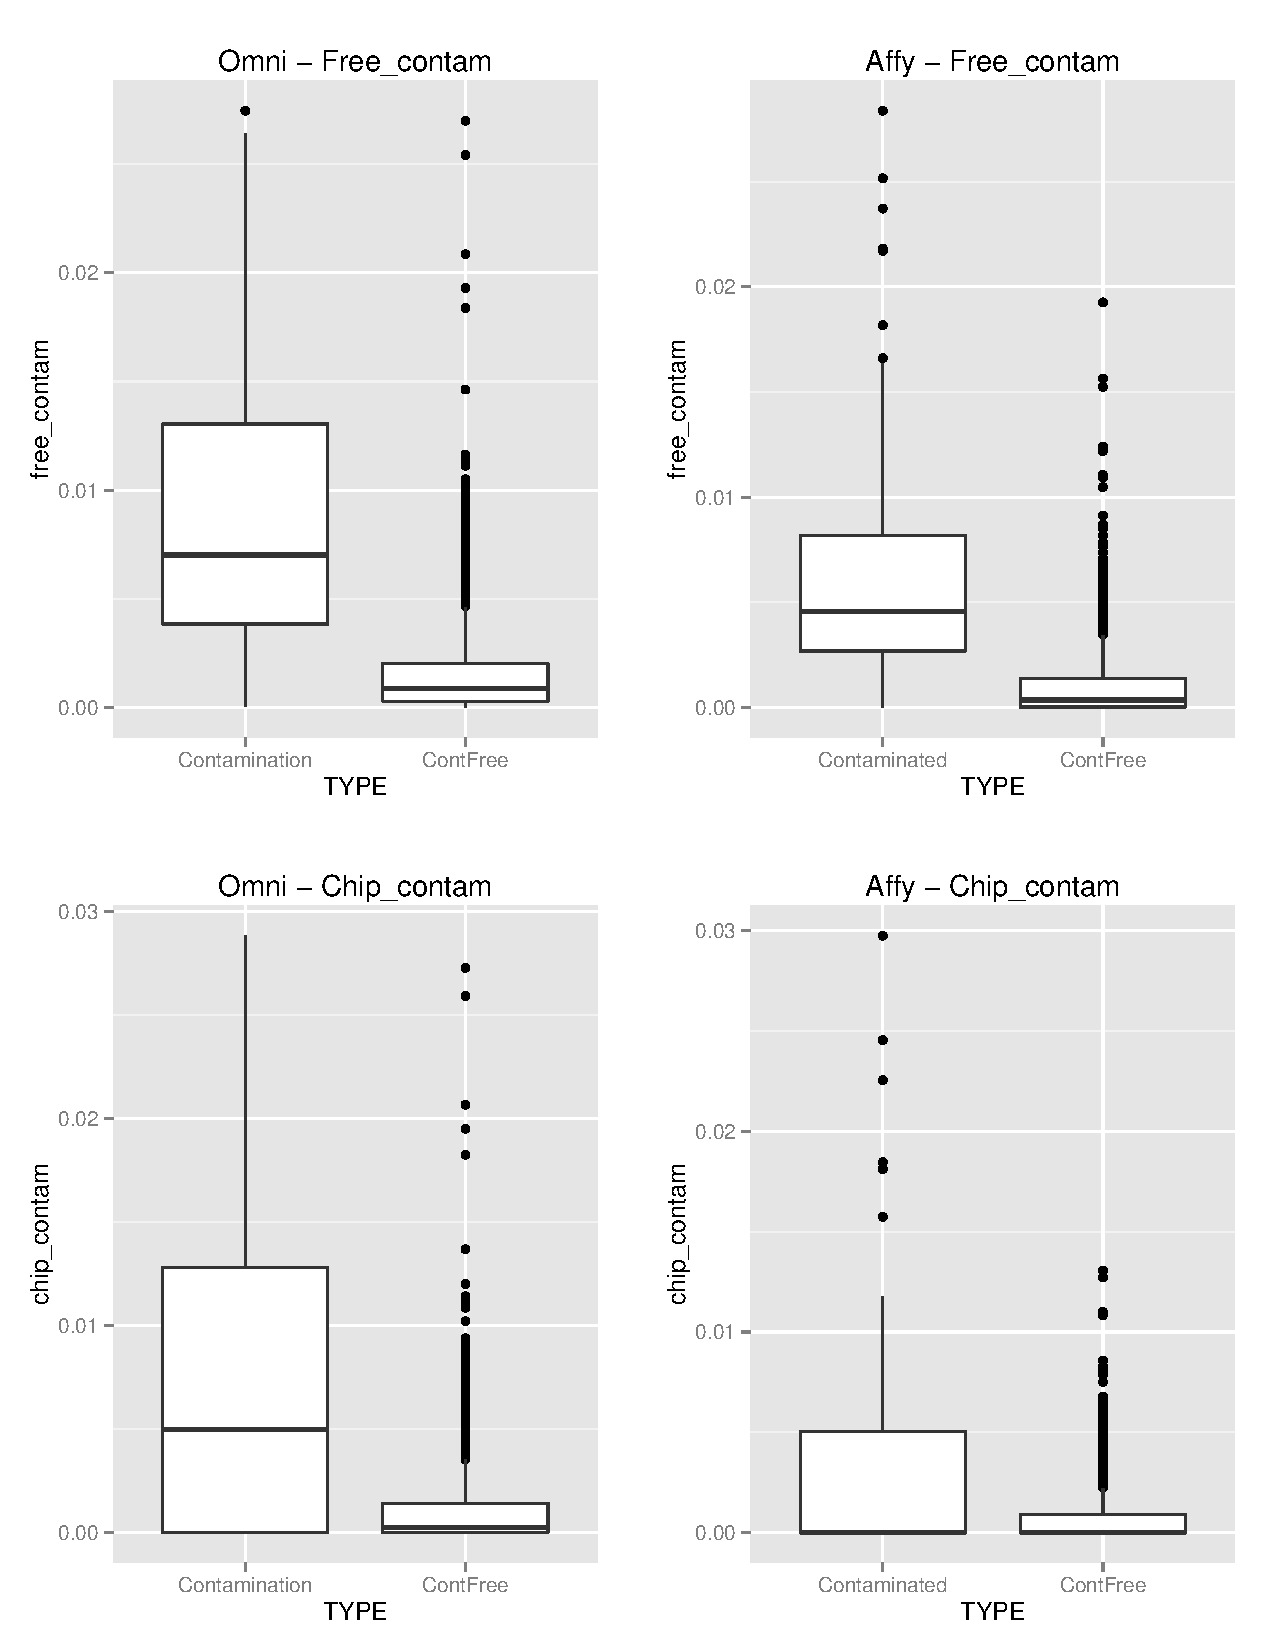
\includegraphics[width=1\textwidth]{images/Result-VerifyBamId-check.pdf}
    \caption[VerifyBamId scores in the contaminated (Contamination) and contamination free (ContFree) Samples]{VerifyBamId scores in the contaminated (Contamination) and contamination free (ContFree) Samples. Omni indicates the scores from VerifyBamId regarding the Illumina Omni Chip, while Affy denotes the Affymetrix Chip scores for VerifyBamId. free\_contam represents the HIGH\_FREE\_MIX, while chip\_contam represents the HIGH\_CHIP\_MIX score}.  
    \label{cont:1000G}
\end{figure}
\end{itemize}

\section{Conclusion and Outlook}\label{cont:outlook}
There are many examples in the literature showing the negative impact of sequencing errors in mtDNA datasets in different areas of research. Standard DNA sequencing procedures are now being replaced by MPS technologies, that are able to retrieve huge amount of sequencing data from biological specimens in a cost-effective manner and short-time span. The arrival of these new technologies is not without problems (\cite{Bandelt2012a}, \cite{Just2015}). The method presented in this Chapter called Haplochecker is a step-forward in the analysis of mtDNA data derived from MPS and it allows preventing sequencing errors and spurious findings. The concept here is to combine the information distilled from the known worldwide phylogeny, based on 24,275 complete humnan mitochondrial DNA sequences\footnote{mtDNA tree Build 17 (18 Feb 2016)\url{http://phylotree.org/}}, providing the database of over 5,400 entries. This database is handled with the JAVA based HaploGrep, by managing the XML-tree directly in memory, read once per instantiation. 

The limitations of the herein presented method are described in Dickins et al \cite{Dickins2014}, but also highlighting the advantage of this approach. The advantage is that contamination can be identified from any source, while already one sample can be analyzed with the entries in the current database, the limitations are identified subsequently:
\begin{itemize}
\item Unavailable haplotypes: This can be indeed of limitation, and the approach here presented highly relies on the data present in the database. There is a clear publication bias in favor to european and asian mtDNA sequences, while african and native american sequences are underrepresented \cite{Fendt2011}. Therefore the limitation will affect merely populations in such branches. 
\item Costly implementation: the authors highlight the relatively costly implementation of a search across a large panel of samples. However we have shown in the Chapter HaploGrep \ref{chapterHaplogrep}, that a query against the in-memory database could be optimized, and the increase of database size follows a linear increase of the run-time. Therefore this limitation is no longer given.
\item Increasing number of haplotypes: the authors argue, that an increase in the number of possible haplotypes and samples increases, leading to a challenging interpretation of the output. As shown with the validation of the 1000G phase 3 dataset, it is also feasible to detect contamination in a set of 2,504 whole genome mtDNA sequences. Projects such as the 100,000 Genome Project\footnote{\url{https://www.genomicsengland.co.uk/the-100000-genomes-project/}} are surely a challenge, but the detection of contamination can be applied also on a per-sample approach, while with the approach of Dickson all sequences need to be in the evaluation, to confirm the contamination, what clearly can be of a challenge in the interpretation of contamination. 
\end{itemize}

While there do exist methods to detect contamination in MPS studies, the herein presented method represents an additional tool for this purpose. Based on various datasets, we could show that the method reliably detects the presence of additional mtDNA profiles, which can be contained to an extent in the 1\% of all reads. 
In addition, it should be denoted, that bioinformatic settings are important for the analysis of high-throughput data and suggest that MPS technologies need further calibration.

